\subsection{Projektstyring}


\subsection{Problemidentifikation}
Af de givne projektoplæg, har vi valgt at fokusere op det trejde projektoplæg (Når hdverdagen rystes), da dette ser ud til at være det mest spændende for os, da det passer ind i vores interesse og vores kompetencer.





\begin{figure}[h]
    \centering
    \fbox{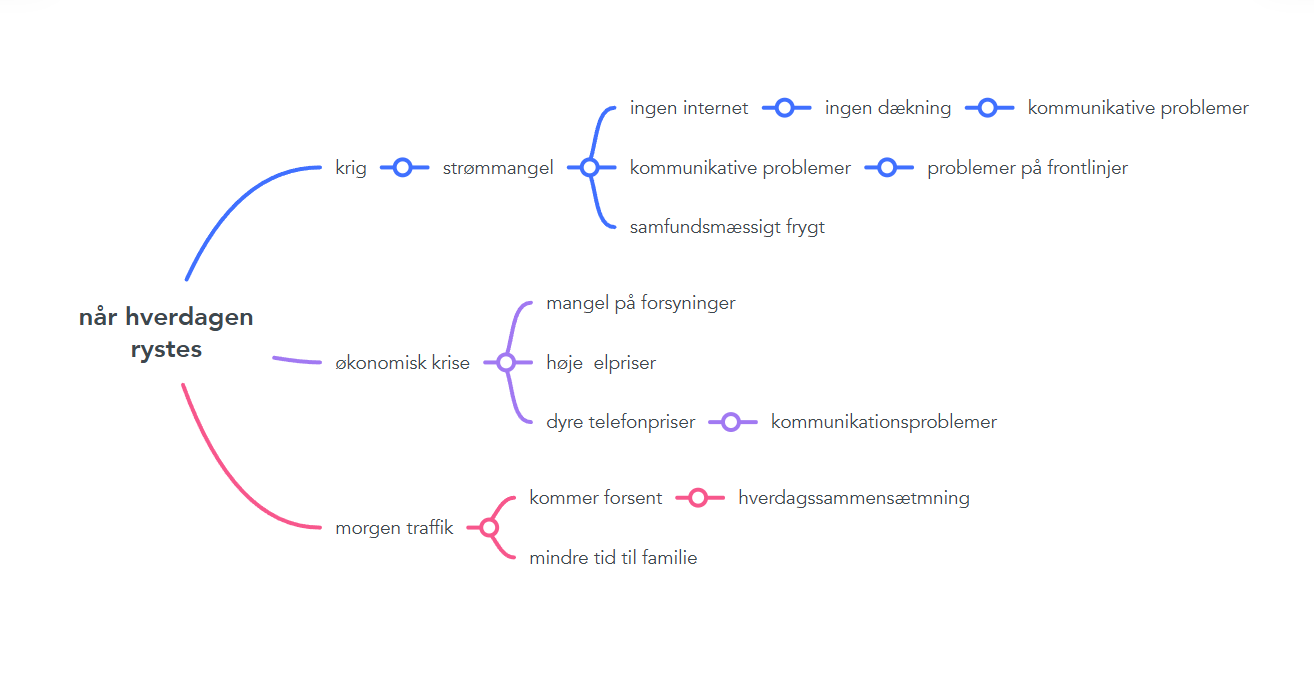
\includegraphics[width=\textwidth]{images/problem-identification.png}}
    \caption{Problemidentifikation}
\end{figure}


I dette projekt, har vi valgt at arbejde med den følgende problemstilling:

Efter ukrainekrigens udbrud i 2022, har verdensbilledet ændret sig markant, det ses bla. ved at beredskabsstyrelsen har lancerert helt kontrete retningslinjer til hvordan danskerne kan forberede sig til eventuelle krisesituationer, som kunne opstå.